\documentclass{IMTexam}

\usepackage[enums]{IMTtikz}
\usepackage{booktabs}
\usepackage{stackengine,collcell}
\let\endminwd\relax
%\newcolumntype{L}[1]{>{\collectcell\xminwd l{#1}$}l<{$\endminwd\endcollectcell}}
\newcolumntype{C}[1]{>{\collectcell\xminwd c{#1}$}c<{$\endminwd\endcollectcell}}
%\newcolumntype{R}[1]{>{\collectcell\xminwd r{#1}$}r<{$\endminwd\endcollectcell}}
\def\minwd#1#2#3\endminwd{\stackengine{0pt}{#3}{\rule{#2}{0pt}}{O}{#1}{F}{F}{L}}
\newcommand\xminwd[1]{\minwd#1}

\givecredits
\author{Isabella B. Amaral}
\USPN{11810773}
\lecture{Matemática II}
\examname{Prova II}
\hwtype{Resolução}
\lcode{}
\date{20 de junho}

\newtheorem{definition}{Definição}
\newtheorem{theorem}{Teorema}[question]
\newtheorem{corollary}{Corolário}[theorem]
\newtheorem{lemma}[theorem]{Lema}
\let\oldemptyset\emptyset
\let\emptyset\varnothing
\newcommand\restrict[1]{{% we make the whole thing an ordinary symbol
        \left.\kern-\nulldelimiterspace % automatically resize the bar with \right
        % the function
        \vphantom{\big|} % pretend it's a little taller at normal size
        \right|_{#1} % this is the delimiter
}}
\DeclarePairedDelimiter\ceil{\lceil}{\rceil}
\DeclarePairedDelimiter\floor{\lfloor}{\rfloor}

\newcommand{\decSep}{,}
\newcommand{\decNum}[3]{\rlap{\ensuremath{\phantom{#1\mathord{\decSep}#2}\overline{\phantom{#3}}}}\num{#1.#2#3}}
%\newcommand{\decSI }[4]{\rlap{\ensuremath{\phantom{#1\mathord{\decSep}#2}\overline{\phantom{#3}}}}\SI{#1.#2#3}{#4}}


\begin{document}

    \maketitle

    \begin{questions}
        \question Demonstre que $\mathrm{e}^2$ é irracional.

        \begin{solution}
            Primeiro mostraremos que $\mathrm{e}$ é irracional, como segue:

            Seja
            \[S_n\coloneq\sum_{k=0}^n\dfrac{1}{k!}.\]
            \begin{lemma}
                Para todo $n>0$ vale que $\mathrm{e}-S_n<1/n!$.
            \end{lemma}
            \begin{proof}
                Pela expansão de Taylor do número de euler, temos que
                \begin{align*}
                    \mathrm{e}-S_n&=\dfrac{1}{(n+1)!}+\dfrac{1}{(n+2)!}+\cdots\\
                    &=\dfrac{1}{n!\cdot(n+1)}+\dfrac{1}{n!\cdot(n+1)(n+2)}+\cdots\\
                    &=\dfrac{1}{n!}\del{\dfrac{1}{(n+1)}+\dfrac{1}{(n+1)(n+2)}+\cdots}\\
                    \intertext{o que, definitivamente, é menor do que $1/n!$ vezes a série geométrica}
                    &<\dfrac{1}{n!}\del{\dfrac{1}{2}+\dfrac{1}{2\cdot 2}+\cdots}\\
                    &<\dfrac{1}{n!}\sum_{k=0}^\infty\dfrac{1}{2^k}\\
                    &<\dfrac{1}{n!}.
                \end{align*}
            \end{proof}

            Agora, suponha que $\mathrm{e}$ é racional, isto é, podemos escrevê-lo como $p/q$ para
            $p,q\in\mathbb{Z}$, dessa forma, pelo lema acima
            \[ \dfrac{p}{q}-S_q<\dfrac{1}{q!}, \]
            porém, fazendo
            \begin{align*}
                \dfrac{p}{q}-S_q&=\dfrac{p}{q}-\del{1+1+\dfrac{1}{2!}+\dfrac{1}{3!}+\cdots}\\
                &=\dfrac{p(q-1)!}{q!}-\dfrac{q!}{q!}-\dfrac{q!}{q!}-\dfrac{q(q-1)\cdots4\cdot3}{q!}-\dfrac{q(q-1)\cdots4}{q!}-\cdots-\dfrac{q}{q!}-\dfrac{1}{q!}\\
                \dfrac{p}{q}-S_q&=\dfrac{C}{q!},\quad C\in\mathbb{Z}
            \end{align*}
            o que implica em
            \[\dfrac{p}{q}-S_q=\dfrac{C}{q!}<\dfrac{1}{q!}\implies C\leqslant 0 \implies \mathrm{e}\leqslant S_n, \]
            o que contradiz nosso lema e nossa intuição.

            Agora, seguindo disso, notamos que a expansão de Taylor de $\mathrm{e}^2$ nos dá
            \[ \mathrm{e}^2 =1+\dfrac{2^1}{1!}+\dfrac{2^2}{2!}+\cdots+\dfrac{2^n}{n!}+\dfrac{2^{n+1}}{(n+1)!}+\cdots \]
            de tal forma que, se $\mathrm{e}^2=p/q$ teremos que
            \[ n!p=n!q\,\mathrm{e}^2=n!q\del{1+\dfrac{2^1}{1!}+\dfrac{2^2}{2!}+\cdots+\dfrac{2^n}{n!}}+q\del{\dfrac{2^{n+1}}{(n+1)}+\cdots}\implies n!p=qS+qR \]
            onde $R$ e $S$ denotam as respectivas parcelas da soma.

            Podemos notar que na formulação acima $n!p$ e $S$ são inteiros, o que implica que $R$ também o seja, porém, para $n>1$ temos
            \[ R=2^{n+1}\del{\dfrac{1}{(n+1)}+\dfrac{1}{(n+1)(n+2)}+\cdots}<2^{n+1}\del{\dfrac{1}{(n+1)}+\dfrac{1}{(n+1)^2}+\cdots}=2^{n+1}\cdot\dfrac{\dfrac{1}{n+1}}{1-\dfrac{2}{n+1}}=\dfrac{2^{n+1}}{n-1} \]
            de tal forma que
            \[ \dfrac{2^{n+1}}{n+1}<R<\dfrac{2^{n+1}}{n-1}. \]
            Agora, analisando $S$ temos
            \[ S=n!\del{1+\dfrac{2}{1!}+\dfrac{2^2}{2!}+\cdots+\dfrac{2^n}{n!}}=\sum_{k=0}^n2^k\cdot\dfrac{n!}{k!}. \]
            Analisando agora as potências de 2 presentes em $n!$ temos a soma
            \[ \left\lfloor\dfrac{n}{2}\right\rfloor+\left\lfloor\dfrac{n}{2^2}\right\rfloor+\cdot +1\leqslant \dfrac{n}{2}+\dfrac{n}{2^2}+\cdots=n \]
            \paragraph{Note que:} cada termo $n/2^\ell$ da soma representa os a quantidade de números $<n$ que possuem $2^\ell$ em sua fatoração.

            Dessa forma, nota-se que a maior potência de $2$ em $n!$ seria $n$, o que de fato só ocorre quando o próprio $n$ é potência de $2$. Tomando $n=2^m$, temos
            \[ \left\lfloor\dfrac{2^m}{2}\right\rfloor+\left\lfloor\dfrac{2^m}{2^2}\right\rfloor+\cdot +2+1 = 2^m - 1 = n-1 \]
            de tal forma que a maior potência de 2 em $2^k\cdot n!/k!$ é pelo menos $k+n-1-k=n-1$. Sendo assim $2^{n-1}|S$, assim como $2^{n-1}|n!p$, portanto, podemos analisar
            \[ \dfrac{n!p}{2^{n-1}}=q\cdot\dfrac{S}{2^{n-1}}+q\cdot\dfrac{R}{2^{n-1}}\implies A=q\cdot S'+q\cdot R' \]
            onde todos os termos permanecem inteiros.

            Retomando os limites derivados anteriormente para $R$, temos, pelo raciocínio acima, que
            \[ 0<\dfrac{1}{2^{n-1}}\dfrac{2^{n+1}}{n+1}<\dfrac{1}{2^{n-1}}R<\dfrac{1}{2^{n-1}}\dfrac{2^{n+1}}{n-1}\implies 0<\dfrac{4q}{n+1}<qR'<\dfrac{4q}{n-1} \]
            e, se $n>4q-1$, segue que $0<qR'<1$ o que nos mostra que $qR'$ não pode ser inteiro e, por consequência, $b$ não o pode ser. Contradição!

            \hfill\qedsymbol
        \end{solution}

        \question Calcule os limites abaixo:

        \begin{parts}
            \part \[ \lim\limits_{x\to\pi} \dfrac{\log|\sin x|}{\log{|\sin 2x|}}. \]

            \begin{solution}
                Como $\sin x$ e $\sin 2x$ tendem à zero conforme $x$ tende à
                $\pi$, e $\log g(x)$ com $g(x)$ tendendo à zero tende à
                $-\infty$, temos uma indeterminação de $0/0$, e podemos usar
                l'hôpital:

                \[ \lim\limits_{x\to\pi} \dfrac{\log|\sin x|}{\log{|\sin 2x|}}=\lim\limits_{x\to\pi} \dfrac{\dod{}{x}\sbr{\log|\sin x|}}{\dod{}{x}\sbr{\log{|\sin 2x|}}}. \]

                sendo o valor absoluto um operador que gera descontinuidades, devemos modificar o formato da função para poder derivá-la:
                \[ \envert{f(x)}=\dfrac{f(x)}{|f(x)|}f(x) \]
                note que: a razão agora é apenas uma forma de extrair o sinal da
                função, de tal forma que se $f(x)<0$, a razão também é negativa
                e os sinais se cancelam no produto das duas. Se o sinal for
                positivo ele é mantido.

                Dessa forma, temos:

                \begin{align*}
                    \lim\limits_{x\to\pi} \dfrac{\log|\sin x|}{\log{|\sin
                    2x|}}&=\lim\limits_{x\to\pi} \dfrac{\dfrac{\sin x}{|\sin
                    x|}\dod{}{x}\sbr{\sin x}/|\sin x|}{\dfrac{\sin 2x}{|\sin
                    2x|}\dod{}{x}\sbr{\sin 2x}/|\sin 2x|}\\[1em]
                    &=\lim\limits_{x\to\pi} \dfrac{\dfrac{\sin x}{|\sin
                    x|}\dfrac{\cos x}{|\sin x|}}{\dfrac{\sin 2x}{|\sin
                    2x|}\dfrac{2\cos 2x}{|\sin 2x|}}\\
                    \intertext{agora, notamos que a multiplicação de módulos iguais nos dá $|f(x)|^2=|(f(x))^2|=(f(x))^2$, dessa forma, temos}
                    &=\lim\limits_{x\to\pi} \dfrac{\sin x\cos x}{2\sin 2x\cos 2x}\\
                    &=\lim\limits_{x\to\pi} \dfrac{\sin 2x}{2\sin 4x}\\
                    \intertext{novamente, temos uma indeterminação de $0/0$ e, portanto, aplicamos l'hôpital novamente}
                    &=\lim\limits_{x\to\pi} \dfrac{\cos 2x}{4\cos 4x}\\
                    \intertext{é fácil notar que $\lim\limits_{x\to\pi}\cos 2n\,x=-1,x\in\mathbb{Z}$ de tal forma que temos}
                    \lim\limits_{x\to\pi} \dfrac{\log|\sin x|}{\log{|\sin 2x|}}&=\dfrac{1}{4}
                \end{align*}
            \end{solution}

            \part \[ \lim\limits_{x\to+\infty} \dfrac{\sin \frac{1}{ax}}{\arctan
            \frac{1}{bx}},\quad\textup{em que }a>0\textup{ e }b>0. \]

            \begin{solution}
                Sabemos que
                $1/(\alpha\,x)\overset{x\to\infty}{\longrightarrow}0$ de tal
                forma que avaliamos a razão de $\sin x/\arctan x$ com $x\to0$, o
                que nos dá uma indeterminação de $0/0$, de tal forma que podemos
                aplicar l'hôpital:
                \[ \lim\limits_{x\to+\infty} \dfrac{\sin \frac{1}{ax}}{\arctan
                \frac{1}{bx}}=\lim\limits_{x\to+\infty} \dfrac{\dod{}{x}\sin
                \dfrac{1}{ax}}{\dod{}{x}\arctan \dfrac{1}{bx}} \]

                Agora, utilizando a propriedade da inversa podemos calcular a
                derivada de $\arctan x$:
                \[ \tan\arctan x=x\implies\dod{}{x}\sbr{\tan\arctan x}=1\implies
                \del{\arctan x}'=\dfrac{1}{\tan' \arctan x} \]
                fazendo a derivada da $\tan x$, temos
                \[ \dod{}{x}\sbr{\dfrac{\sin x}{\cos x}}=\dfrac{\cos^2 x -
                \del{-\sin^2 x}}{\cos^2 x}=1+\tan^2 x \]
                dessa forma:
                \[ \arctan' x = \dfrac{1}{1 +\del{\tan{\arctan
                x}}^2}=\dfrac{1}{1+x^2}. \]

                Portanto:
                \begin{align*}
                    \lim\limits_{x\to+\infty} \dfrac{\sin \frac{1}{ax}}{\arctan \frac{1}{bx}}&=\lim\limits_{x\to+\infty} \dfrac{\dod{}{x}\sin \dfrac{1}{ax}}{\dod{}{x}\arctan \dfrac{1}{bx}}\\
                    &=\lim\limits_{x\to+\infty}\dfrac{-x^{-2}/a\cos (1/ax)}{-x^{-2}/b\del{1+1/(bx)^2}^{-1}}\\
                    &=\lim\limits_{x\to+\infty}\dfrac{b\cos (1/ax)((bx)^2+1)}{a(bx)^2}\\
                    &=\lim\limits_{x\to+\infty}\dfrac{b}{a}\cos \del{\dfrac{1}{ax}}+\dfrac{b}{a}\dfrac{\cos (1/ax)}{(bx)^2}\\
                    &=\lim\limits_{x\to+\infty}\dfrac{b}{a}\cos \del{\dfrac{1}{ax}}+\lim\limits_{x\to+\infty}\dfrac{b}{a}\cos\del{\dfrac{1}{ax}}\dfrac{1}{(bx)^2}\\
                    \intertext{como $1/x$ tende à zero conforme $x$ tende ao infinito, temos dois limites nulos}
                    \lim\limits_{x\to+\infty} \dfrac{\sin \frac{1}{ax}}{\arctan \frac{1}{bx}}&=0.
                \end{align*}
            \end{solution}

            \part \[ \lim\limits_{x\to 0^{-}}(1-4^x)^{\sin 2x}. \]

            \begin{solution}
                Tomando a exponencial, podemos então fazer

                \[ \lim\limits_{x\to 0^{-}}(1-4^x)^{\sin 2x}=\lim\limits_{x\to 0^{-}}\exp\del{\ln{(1-4^x)^{\sin 2x}}} \]
                agora avaliamos o limite do expoente:
                \[ \lim\limits_{x\to 0^{-}}\sin 2x\ln{1-4^x}=0 \]
                dessa forma, temos
                \[ \lim\limits_{x\to 0^{-}}(1-4^x)^{\sin 2x}=\mathrm{e}^0=1. \]
            \end{solution}

            \part \[ \lim\limits_{x\to
            0}\del{\dfrac{1}{\log(x+\sqrt{1+x^2})}-\dfrac{1}{\log(1+x)}} \]

            \begin{solution}
                Tomando o mínimo denominador comum da subtração, temos
                \[ \lim\limits_{x\to 0}\del{\dfrac{1}{\log(x+\sqrt{1+x^2})}-\dfrac{1}{\log(1+x)}}=\lim\limits_{x\to 0}\dfrac{\log\del{1+x}-\log\del{x+\sqrt{1+x^2}}}{\log(x+\sqrt{1+x^2})\log(1+x)} \]
                dessa forma, temos um limite indeterminado de $0/0$ e, por l'hôpital, temos

                \begin{align*}
                    \lim\limits_{x\to 0}\dfrac{\log\del{1+x}-\log\del{x+\sqrt{1+x^2}}}{\log(x+\sqrt{1+x^2})\log(1+x)}
                    &=\lim\limits_{x\to 0}
                    \dfrac{
                        \dfrac{1}{1+x}-\del{\dfrac{\sqrt{1+x^2}+x}{\sqrt{1+x^2}}}\dfrac{1}{x+\sqrt{1+x^2}}
                    }{
                        \dod{}{x}\sbr{\log(x+\sqrt{1+x^2})\log(1+x)}
                    }\\
                    &=\lim\limits_{x\to 0}
                    \dfrac{
                        \dfrac{1}{1+x}-\dfrac{1}{\sqrt{1+x^2}}
                    }{
                        \dfrac{\log(1+x)}{\sqrt{1+x^2}}+\dfrac{\log(x+\sqrt{1+x^2})}{1+x}
                    }\\
                    &=\lim\limits_{x\to 0}
                    \dfrac{
                        \dfrac{\sqrt{1+x^2}-(1+x)}{(x+1)\sqrt{1+x^2}}
                    }{
                        \dfrac{\log(1+x)(x+1)+\log(x+\sqrt{1+x^2})\sqrt{1+x^2}}{(x+1)\sqrt{1+x^2}}
                    }\\
                    &=\lim\limits_{x\to 0}
                    \dfrac{
                        \sqrt{1+x^2}-(1+x)
                    }{
                        \log(1+x)(x+1)+\log(x+\sqrt{1+x^2})\sqrt{1+x^2}
                    }\\
                    \intertext{o que ainda nos dá um limite indeterminado da forma $0/0$, portanto, aplicamos l'hôpital novamente}
                    &=\lim\limits_{x\to 0}
                    \dfrac{
                        \dfrac{x}{\sqrt{1+x^2}}-1
                    }{
                        1+\log(x+1)+1+\log(x+\sqrt{1+x^2})\dfrac{x}{\sqrt{1+x^2}}
                    }\\
                    \lim\limits_{x\to 0}\dfrac{\log\del{1+x}-\log\del{x+\sqrt{1+x^2}}}{\log(x+\sqrt{1+x^2})\log(1+x)}
                    &=-\dfrac{1}{2}.
                \end{align*}
            \end{solution}

            \part \[ \lim\limits_{x\to0^{-}}\dfrac{1}{x\sqrt{x}}\del{a\arcsin
            \dfrac{\sqrt{x}}{a}+b\arcsin{\dfrac{\sqrt{x}}{b}}},\quad\textup{com
            }a>b>0. \]

            \begin{solution}
                Como a função é indefinida para $x\leqslant 0$, podemos dizer
                com segurança que o limite é indefinido, no entanto, avaliamos o
                limite para $x\to0^{+}$ por motivos de completude:

                Sendo o limite indeterminado ($0/0$), podemos aplicar l'hôpital,
                porém primeiro precisamos da derivada do arco seno. Pela
                propriedade da inversa, temos que:
                \begin{align*}
                    \sin\arcsin x&=x\implies \arcsin' x=\dfrac{1}{\cos\arcsin x}\\
                    \intertext{pela identidade fundamental da trigonometria, temos}
                    \sin\arcsin x&=\dfrac{1}{\sqrt{1-\del{\sin\arcsin x}^2}}=\dfrac{1}{\sqrt{1-x^2}}.
                \end{align*}
                Dessa forma, podemos derivar o numerador e denominador do limite em questão:
                \begin{align*}
                    \lim\limits_{x\to0^{+}}\dfrac{1}{x\sqrt{x}}\del{a\arcsin \dfrac{\sqrt{x}}{a}+b\arcsin{\dfrac{\sqrt{x}}{b}}}
                    &=\lim\limits_{x\to0^{+}}
                    \dfrac{
                        \dfrac{1}{2\sqrt{x}}\del{\dfrac{1}{1-\del{\sqrt{x}/a}^2}+\dfrac{1}{1-\del{\sqrt{x}/b}^2}}
                    }{
                        \dfrac{3}{2}\sqrt{x}
                    }\\
                    &=\lim\limits_{x\to0^{+}}
                    \dfrac{1}{3x}\del{\dfrac{a^2}{a^2-x}+\dfrac{b^2}{b^2-x}}=\infty
                \end{align*}

            \end{solution}
        \end{parts}

        \question Seja $A>1$, determine, se existe tal elemento,
        $c\in\mathbb{R}$ tal que

        \[ \lim\limits_{x\to+\infty}\del{\dfrac{x+c}{x-c}}^x=A. \]

        \begin{solution}
            Manipulando a expressão interna do limite, temos
            \begin{align*}
                \del{\dfrac{x+c}{x-c}}^x&=\del{\dfrac{1+c/x}{1-c/x}}^x=\dfrac{\del{1+c/x}^x}{\del{1-c/x}^x}\\
                \del{\dfrac{x+c}{x-c}}^x&=\dfrac{\mathrm{e}^{\ln\del{1+c/x}^x}}{\mathrm{e}^{\ln\del{1-c/x}^x}}
            \end{align*}
            sendo a expressão dos expoentes da forma $\ln(g(x))/(1/x)$, o que é indeterminado conforme $x$ tende ao infinito, podemos aplicar l'hôpital:
            \[ \lim\limits_{x\to\infty}\dfrac{\ln\del{1+c/x}}{1/x}=\lim\limits_{x\to\infty}\dfrac{\del{-c/x^2}\del{x/(x+c)}}{-1/x^2}=\lim\limits_{x\to\infty}\dfrac{c\,x}{x+c}=\lim\limits_{x\to\infty}\dfrac{c}{1+c/x}=c \]
            de forma análoga, temos
            \[ \lim\limits_{x\to\infty}\dfrac{\ln\del{1-c/x}}{1/x}=\lim\limits_{x\to\infty}\dfrac{-c}{1-c/x}=-c \]
            portanto, ficamos com
            \[
            \lim\limits_{x\to+\infty}\del{\dfrac{x+c}{x-c}}^x=\lim\limits_{x\to+\infty}\dfrac{\mathrm{e}^{\ln\del{1+c/x}^x}}{\mathrm{e}^{\ln\del{1-c/x}^x}}=\dfrac{\mathrm{e}^{c}}{\mathrm{e}^{-c}}=e^{2c}=A\implies
            c=\dfrac{\ln A}{2}. \]
            e, sendo $A>1$, podemos dizer que existe tal $c$ nos reais.
        \end{solution}

        \question Decida, justificando sua conclusão, se existem reais $a$ e $b$ tais que
        \[ \lim\limits_{x\to0}\dfrac{1}{x-a\tan x}\int_0^x \dfrac{t^2}{\sqrt{b+t}}\dif t=1. \]

        \begin{solution}
            Tomando a integral na expressão temos que
            \begin{align*}
                \int_0^x \dfrac{t^2}{\sqrt{b+t}}\dif t&=\int_b^{b+x} \dfrac{(u-b)^2}{\sqrt{u}}\dif u,\quad\textup{onde } u=b+t\\
                &=\int_b^{b+x} u^{3/2}-2b^2\sqrt{u}+\dfrac{b^2}{\sqrt{u}}\dif u\\
                &=\eval{\del{\dfrac{2}{5}(b+t)^{5/2}-\dfrac{4}{3}b(b+t)^{3/2}+2b^2\sqrt{b+t}}}_0^{x}\\
                &=\eval{\del{\dfrac{2}{15}\sqrt{b+t}\del{3t^2-4b\,t+8b^2}}}_0^{x}\\
                \int_0^x \dfrac{t^2}{\sqrt{b+t}}\dif t&=\dfrac{2}{15}\del{\sqrt{b+x}\del{3x^2-4b\,x+8b^2}-8b^2\sqrt{b}}
            \end{align*}

            Dessa forma, há
            \begin{align*}
                \lim\limits_{x\to0}\dfrac{1}{x-a\tan x}\int_0^x \dfrac{t^2}{\sqrt{b+t}}\dif t
                &=\lim\limits_{x\to0}\dfrac{1/x}{1-(a/x)\tan x}\dfrac{2}{15}\del{\sqrt{b+x}\del{3x^2-4b\,x+8b^2}-8b^2\sqrt{b}}\\
                &=\lim\limits_{x\to0}\dfrac{2}{15}\dfrac{\del{\sqrt{b+x}\del{3x^2-4b\,x+8b^2}-8b^2\sqrt{b}}}{1-(a/x)\tan x}\dfrac{1}{x}\\
                &=\lim\limits_{x\to0}\dfrac{2}{15}\del{8b^2\dfrac{\dfrac{\sqrt{b+x}-\sqrt{b}}{x}}{1-(a/x)\tan x}+\dfrac{\sqrt{b+x}\del{3x-4b}}{1-(a/x)\tan x}}\\
                &=\lim\limits_{x\to0}\dfrac{2}{15}\del{8b^2\dfrac{\dfrac{1}{\sqrt{b+x}+\sqrt{b}}}{1-(a/x)\tan x}+\dfrac{\sqrt{b+x}\del{3x-4b}}{1-(a/x)\tan x}}\\
                &=\dfrac{2}{15}\del{8b^2\dfrac{\dfrac{1}{\sqrt{b}+\sqrt{b}}}{1-a}-\dfrac{4b\sqrt{b}}{1-a}}\\
                &=\dfrac{2}{15}\del{\dfrac{8b\sqrt{b}-4b\sqrt{b}}{1-a}}\\
                \lim\limits_{x\to0}\dfrac{1}{x-a\tan x}\int_0^x \dfrac{t^2}{\sqrt{b+t}}\dif t&=\dfrac{8}{15}\dfrac{b\sqrt{b}}{1-a}.
            \end{align*}

            Fazendo
            \[ \dfrac{8}{15}\dfrac{b\sqrt{b}}{1-a}\overset{!}{=}1\implies b^{3/2}=\dfrac{15}{8}(1-a), \]
            o que nos mostra que há, de fato, infinitas soluções para o problema proposto.
        \end{solution}

        \question Considere funções $f$ e $g$ definidas em $\intoo{-1,1}$ com valores em
        $\mathbb{R}$, deriváveis em $\intoo{-1,1}\backslash \set{0}$,
        integráveis em qualquer intervalo $\intcc{a,b}\subset\intoo{-1,1}$, com
        $g(x)g'(x)\neq 0$ se $x\neq 0$ e suponha que $f(x)$ é o $o\del{g(x)}$
        para $x\to 0$.

        Decida se as afirmações a seguir são verdadeiras ou falsas, no caso de
        ser verdadeira apresente uma demonstração disso, caso seja falsa exiba
        um contra exemplo (respostas ``secas'' apenas com o veredicto sobre a
        frase enunciada não valerão nota estritamente positiva).

        \begin{parts}
            \part Se $F(x)=\int_0^x f(s) \dif s$ e $G(x)=\int_0^x g(s)\dif s$
            então $F(x)$ é $o\del{G(x)}$ para $x\to0$.

            \begin{solution}
                Tome, por definição, que
                \[ \lim\limits_{x\to0}\dfrac{f(x)}{g(x)}=0, \]
                então, para todo $\varepsilon>0$ existe $0<|x|<\delta<1$ tal que
                \[ \envert{\dfrac{f(x)}{g(x)}}<\varepsilon. \]
                Considerando a desigualdade
                \begin{align*}
                    |F(x)|&\leqslant\int_0^x|f(s)|\dif s\\
                    \intertext{para $G(x)\neq0$ temos que}
                    \envert{\dfrac{F(x)}{G(x)}}&\leqslant\dfrac{\int_0^x|f(s)|\dif s}{\envert{G(x)}} <\dfrac{\varepsilon\int_0^x|g(s)|\dif s}{\envert{G(x)}}\\
                    \intertext{e, no intervalo considerado, vale que
                    $g'(x)\neq0$, de tal forma que $g(x)$ tem sinal constante,
                    portanto vale que}
                    \envert{\dfrac{F(x)}{G(x)}}&<\dfrac{\varepsilon\int_0^x|g(s)|\dif s}{\envert{G(x)}} =\dfrac{\varepsilon\envert{\int_0^x g(s)\dif s}}{\envert{G(x)}}=\varepsilon\\
                    \implies\lim\limits_{x\to0}\dfrac{F(x)}{G(x)}&=0.
                \end{align*}

                \hfill\qedsymbol
            \end{solution}

            \part $f'(x)$ é $o\del{g'(x)}$ para $x\to 0$.

            \begin{solution}
                Seja $g(x)$ a função identidade, defina
                \[f(x)=\begin{cases}
                    x^2\sin\del{\dfrac{1}{x}},&\textup{para } x\neq0\\
                    0,&\textup{para }x=0
                \end{cases},\]
                note que teremos $f(x)=o(g(x))$ com $x\to0$, já que
                \[ \lim\limits_{x\to0}\dfrac{x\del{\dfrac{\sin\del{1/x}}{1/x}}}{x}=0. \]

                Derivando, temos
                \[f'(x)=\begin{cases}
                    2x\sin\del{\dfrac{1}{x}}-\cos\del{\dfrac{1}{x}},&\textup{para } x\neq0\\
                    0,&\textup{para }x=0
                \end{cases},\]
                e, notamos que $f'(x)\neq o(g(x))$, já que
                \[ \lim\limits_{x\to0}2x\sin\del{\dfrac{1}{x}}-\cos\del{\dfrac{1}{x}} \]
                é indefinido.

                \hfill\qedsymbol
            \end{solution}
        \end{parts}

        \question Seja $f\colon \intoo{-1,1}\longrightarrow \mathbb{R}$ com
        $n+1$ derivadas contínuas e considere
        $\theta\colon\intoo{-1,1}\longrightarrow\intoo{0,1}$ uma função tal que,
        se $x\in\intoo{-1,1}$, tem-se
        \[ f(x)=\sum_{k=0}^{n-1}\dfrac{f^{(k)}(0)}{k!}x^k+\dfrac{f^{(n)}(x\,\theta(x))}{n!}x^n. \]

        Prove que existe pelo menos uma função $\theta$ com essa propriedade e
        mostre que, se $f^{(n+1)}(0)\neq 0$, então
        $\lim\limits_{x\to0}\theta(x)=\dfrac{1}{n+1}$.

        \begin{solution}
        \end{solution}

        \question Sejam $f\colon \intcc{a,b}\times\mathbb{R}\longrightarrow
        \mathbb{R}$ contínua e $x_0\in\intcc{a,b}$. Mostrar que
        $\varphi\colon\intcc{a,b}\longrightarrow\mathbb{R}$ é solução do
        problema de Cauchy $y'=f(x,y), y(x_0)=y_0$ se, e somente se,
        $\varphi(x)=y_0+\int_{x_0}^x f(u,\varphi(u))\dif u$, para todo
        $x\in\intcc{a,b}$.

        \begin{solution}
        \end{solution}

        \question Considere a equação diferencial
        \[ x(x-1)y'+y=x^2-1. \]

        Determine todas as soluções dessa equação definidas, respectivamente em
        $\intoo{-\infty,0}, \intoo{0,1}$ e $\intoo{1,\infty}$. Analise os
        limites dessas soluções para $x$ tendendo a $0$ ou a $1$, nos casos em
        que isso fizer sentido.

        \begin{solution}
        \end{solution}

        \question Uma cultura de bactérias é atacada por toxinas produzidas a
        partir do instante $t=0$. O total de toxinas cresce numa razão constante
        $a>0$.

        Na ausência de toxinas o número de bactérias, $x(t)$, cresce com taxa
        $k>0$ diretamente proporcional a $x(t)$, com a presença de toxinas essa
        taxa diminui num número diretamente proporcional ao total de bactérias
        nesse instante.

        \begin{parts}
            \part Justifique porque a equação $x'=x(k-a\,t)$ para algum $k>0$,
            descreve de forma adequada a evolução de $x(t), t\geqslant 0$.

            \begin{solution}
                Sendo a taxa de crescimento da população de bactérias ($x'$)
                diretamente proporcional à quantidade de bactérias no mesmo instante
                ($x$), podemos escrever $x'\propto x\implies x'=k\,x$ onde $k>0$.
                Porém como temos a introdução de uma toxina que afeta negativamente
                esse crescimento, e cuja quantidade é proporcional ao tempo $t$ e à
                quantidade atual de bactérias $x$, temos a quantidade de toxinas
                $To\propto x\,t\implies T=a\,x\,t$ com $a>0$ e, dessa forma, $x'$
                pode ser escrito como a soma do ganho + perda:
                \[ x'=k\,x-To=k\,x-a\,x\,t=x\del{k-a\,t}. \]
            \end{solution}

            \part \textbf{Sem resolver a equação diferencial determinada em
            (i)}, determine o instante de tempo $T>0$ em que $x(t)$ é máximo
            (justifique).

            \begin{solution}
                Pela equação diferencial temos que
                \[ x'=x\del{k-a\,t}\implies x=\dfrac{x'}{k-a\,t} \]
                e quando $k-a\,t\to 0$, $x\to\infty$ (considerando que $x'$ é
                positiva, já que não já população negativa).

                Dessa forma queremos que $T$ aproxime $k/a$.
            \end{solution}

            \part Suponha que em $t=0$ o número de bactérias é $x_0>0$,
            determine $x(t)$ para $t>0$, calcule $x(T)$, em que $T$ foi
            determinado no item anterior, e faça o gráfico dessa função.

            \begin{solution}
                Fazendo $x'=\dod{x}{t}$, temos
                \[ \dod{x}{t}=x(k-a\,t)\implies \dfrac{1}{x}\dif x=\del{x-a\,t}\dif t \]
                onde $\dif x$ e $\dif t$ são diferenciais, integrando, temos
                \[ \int\dfrac{1}{x}\dif x=\int\del{k-a\,t}\dif t\implies \log|x|=k\,t-\dfrac{a}{2}t^2+C\implies x(t)=\exp\del{k\,t-\dfrac{a}{2}t^2+C} \]
                pela condição inicial, temos que
                \[ x(0)=x_0=\exp\del{C}\implies C=\log x_0 \]
                de tal forma que
                \[ x(t)=x_0\exp\del{k\,t-\dfrac{a}{2}t^2}\implies x\del{T=\dfrac{k}{a}}=x_0\exp\del{\dfrac{k^2}{a}-\dfrac{k^2}{2a}}=x_0\exp\del{\dfrac{k^2}{2a}}. \]

                Plotando, temos

                \begin{center}
                    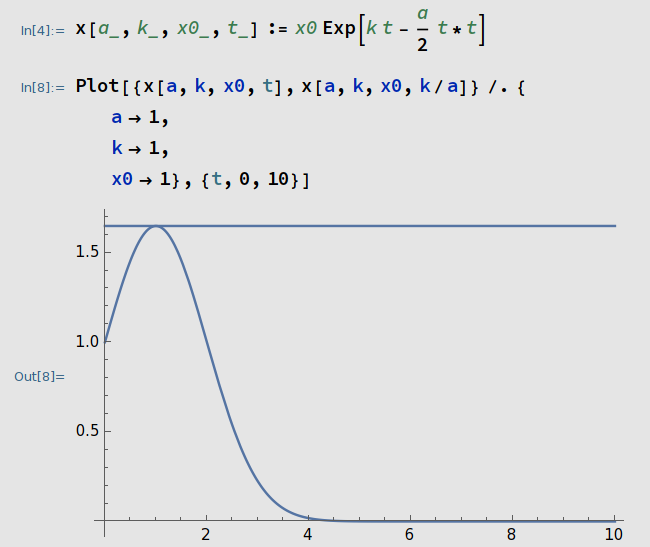
\includegraphics[width=0.8\linewidth]{2021-06-19-18-00-15.png}
                \end{center}

                onde a reta superior (que tangencia o gráfico) representa $x(T)$.

            \end{solution}
        \end{parts}


    \end{questions}
\end{document}
